\chapter{Integrating Unity 3D-Model} \label{sec:unity-integrating-unity-3d-model}

The Smart Home Lab website has been integrated with Unity 3D-Model. Unity is a game engine used to develop computer games and console games for cross-platform devices. With Unity game engine, 2D- and 3D-Model can be built through the provided APIs. The created 3D-Model can be viewed on web browsers through Unity Web Player plugins.

By default, WordPress doesn't have built-in Unity Web Player nor provide any support to view the Unity 3D-Models. Hence, integrating the 3D-Model has to be done manually. This chapter will outline and explain on how to integrate the 3D-Model into a WordPress powered website. Integrating Unity 3D-Model involves 2 steps. First, uploading the Unity files to resource folder. Second, developing a web page to render the 3D-Model.

\section{Uploading Unity Files} \label{sec:unity-uploading-unity-files}
This section will explain how to upload Unity files into WordPress resource folder. The Unity 3D-Model consists of following directories and files as shown below. 
\newline

\dirtree{%
.1 /.
.2 Build.
.3 Prototyp\_V2\_Web.asm.code.unityweb.
.3 Prototyp\_V2\_Web.asm.framework.unityweb.
.3 Prototyp\_V2\_Web.asm.memory.unityweb.
.3 Prototyp\_V2\_Web.data.unityweb.
.3 Prototyp\_V2\_Web.json.
.3 UnityLoader.js.
.2 TemplateData.
.3 favicon.ico.
.3 fullscreen.png.
.3 progressEmpty.Dark.png.
.3 progressEmpty.Light.png.
.3 progressFull.Dark.png.
.3 progressFull.Light.png.
.3 progressLogo.Dark.png.
.3 progressLogo.Light.png.
.3 style.css.
.3 UnityProgress.js.
.3 webgl-logo.png.
}

\bigskip

These files has to be uploaded to the directory \begin{quote}\path{/var/www/html/wp-content/uploads/}\end{quote} in the server. Uploading those 2 directories together with the files is done through \texttt{git clone} method. Fisrt, these files have been uploaded to a git repository. There is no any specific git account or git repository has been created for the Smart Home Lab website purpose. Please use your own or create one for the website if it is necessary.

After uploading 3D-Model files into a git repository, login into the backend of the server using PuTTY with hostname and port number as shown in the Figure~\ref{fig:login-putty}. Don't forget to include the \texttt{private\_key.ppk} for authentication under \texttt{Auth} tab in the PuTTY. Once the session is opened, enter the SSH passphrase \texttt{BSY2qjtu\$\#}

\begin{figure}[h]
\caption{Login into backend using PuTTY}
\label{fig:login-putty}
\centering
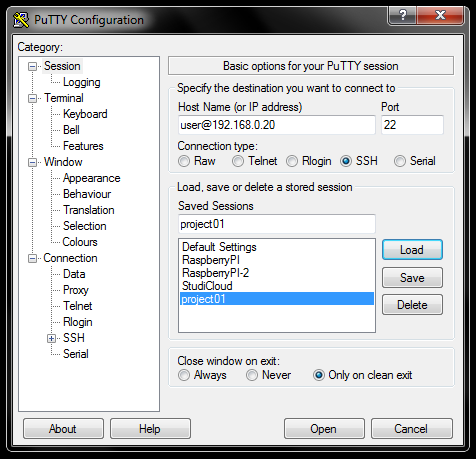
\includegraphics[width=.5\linewidth,keepaspectratio]{unity/putty.png}
\end{figure}

Navigate to the directory \texttt{/var/www/html/wp-content/uploads}. And use \texttt{git clone} method to clone i.e. download the required Unity 3D-Model files to the server. Replace the \texttt{[url]} with the URL address of the git repository.

\begin{lstlisting}
cd /var/www/html/wp-content/uploads
git clone [url]
\end{lstlisting}

Since the directories and files are uploaded through the system user of Ubuntu Server, by default WordPress don't have permission to access them. File ownership and file permission for those directories and files has to set using \texttt{chown} and \texttt{chmod}.

\begin{lstlisting}
chown -R user:www-data /var/www/html/wp-content/uploads/Build
chown -R user:www-data /var/www/html/wp-content/uploads/TemplateData
chmod -R g+w /var/www/html/wp-content/Build
chmod -R g+w /var/www/html/wp-content/TemplateData
\end{lstlisting}

Uploading the required Unity 3D-Model is done with setting of file ownership and file permission. In the next section, the rendering of HTML page will discussed and explained.

\section{Rendering HTML for Unity Web Player} \label{sec:unity-rendering-html-for-unity}
This section will discuss on adding the HTML tag to render the Unity Web Player as well as linking the required Unity 3D-Model files, that have been uploaded to web server directory as discussed in the Section~\ref{sec:unity-uploading-unity-files}.

First, a new web page has to be added by using the WordPress built-in Page function. Click on 'Pages' option from the side menu and 'Add New' sub option. Here, '3D Model' has been given as the title of the page with \texttt{/unity} as the relative web page path.

In the editor column, HTML codes have been added to render the Unity Web Player. The web player will be rendered inside 2 \texttt{div} containers with class names \texttt{webgl-content} and \texttt{gameContainer} respectively. However, the web player is fixed to size of 960 pixel width and 600 pixel height as set by the author of the 3D-Model. This attributes have not been changed. Fixing the width and height will cause the page not to act responsively across various screen sizes. Codes snippet below shows the rendering of Unity Web Player.

\begin{lstlisting}
<div class="webgl-content" style="margin-top: 17%; margin-bottom: 10%">
    <div id="gameContainer" style="width: 960px; height: 600px"></div>
    <div class="footer">
        <div class="webgl-logo"></div>
        <div class="fullscreen" onclick="gameInstance.SetFullscreen(1)"></div>
        <div class="title">Smart-Home-Labor</div>
     </div>
</div>
\end{lstlisting}

Next, required files has to be linked to web page. These files include \texttt{style.css}, \texttt{UnityProgress.js}, and \texttt{UnityLoader.js}. These files are included onto the web page as shown in code snippet below.

\begin{lstlisting}
// linking required files
<link rel="stylesheet" href="../wp-content/uploads/TemplateData/style.css">
<script src="../wp-content/uploads/TemplateData/UnityProgress.js"></script>  
<script src="../wp-content/uploads/Build/UnityLoader.js"></script>
\end{lstlisting}

After that, the web player has to instantiated using the \texttt{UnityLoader.instantiate()} function.

\begin{lstlisting}
<script>
	const gameInstance = UnityLoader.instantiate(
		"gameContainer",
		"../wp-content/uploads/Build/Web_V6.json",
		{
			onProgress: UnityProgress
		}
	);
</script>
\end{lstlisting}

Lastly, in order to enhance the user interface level, the title of the web page has to be removed. This ensures that the Unity Web Player uses the maximum space in the view. The default title of the web page is removed by using CSS code as shown below. This code has be inserted into 'Scripts n Styles' column under 'Styles' tab.

\begin{lstlisting}
.entry-header {
	display: none;
}
\end{lstlisting}

\section{Alternative way to upload Unity 3D-Model Files}
Another alternative way to upload the required Unity 3D-Model files is by using the 'File Manager' plugin\footnote{https://wordpress.org/plugins/file-manager/}. This plugin is available free of cost in the WordPress plugins directory\footnote{https://wordpress.org/plugins/}. This plugin can be added to the website and activate through the web browser.

\begin{figure}[h]
\caption{File Manager Plugin}
\label{fig:file-manager-screen}
\centering
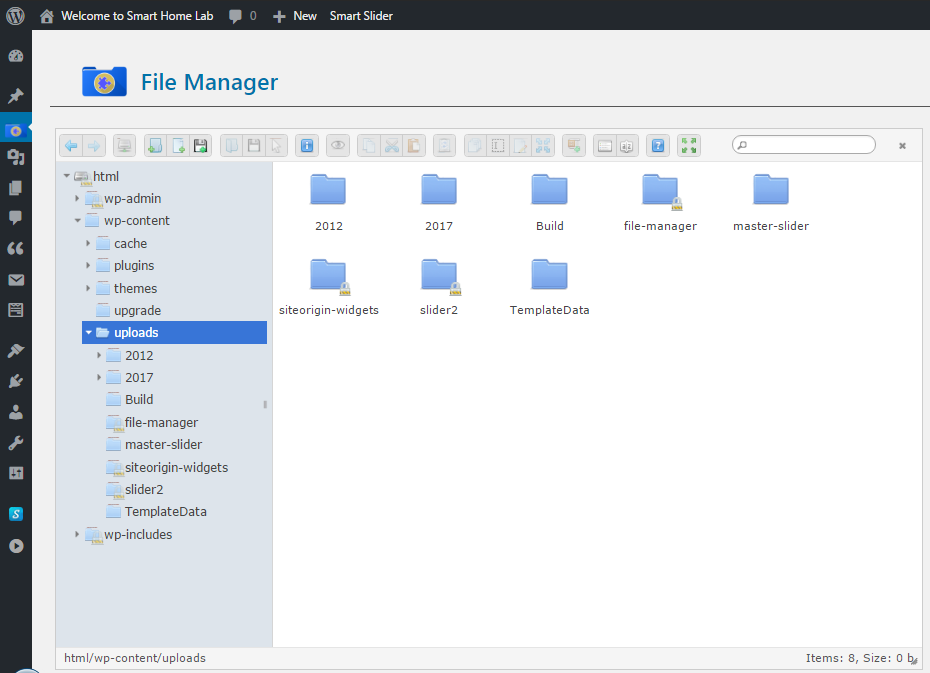
\includegraphics[width=.65\textwidth,keepaspectratio]{unity/file-manager-plugin.png}
\end{figure}

After installation and activation of this plugin, a new 'File Manager' option will appear on the left menu bar. This plugin enables the directories and files on the backend server to be viewed on the front-end web interface (see Figure~\ref{fig:file-manager-screen}).

Through this plugin, directories and files can be added, modified and deleted. Here, the root directory starts with \texttt{/html/.}, instead of \texttt{/var/www/html/.}. The \texttt{html} is the root directory of WordPress where else \texttt{/var/www} is the root directory of the Nginx web server.

Uploading file through 'File Manager' plugin can be done simply by drag-n-drop method. The files, however, have to made sure uploaded to the correct directory, which is \texttt{/html/wp-content/uploads}. Since we used WordPress frontend to upload the files, no file ownership and file permission has to be set. Here the files and directories are added with WordPress as the owner.

Even though this method is much simpler than the method discussed in the Section~\ref{sec:unity-uploading-unity-files}, a problem has occurred. There is a file with size of almost 12 MB in the \texttt{TemplateData} directory. This file are not uploading to the server by using the 'File Manager' plugin. The WordPress deliver a \texttt{http-error}. After research and studies, no working solution has been found on how to enable large file upload of more than 10 MB.

This is taking into consideration after increasing the file upload size limit both in the Nginx web server configuration and PHP application server configuration. Solving the \texttt{http-error} will enable the file to uploaded or upgraded easily in the future by using this plugin, without having to login in to server backend and uploading file using PuTTY or SFTP.
